\documentclass{jreport}
\usepackage{ulem}
\usepackage{xcolor}
\usepackage{amsmath}
\usepackage{amsfonts}
\usepackage{amssymb}
\usepackage{amsthm}
\usepackage{bm}
\usepackage{romannum}
\usepackage[dvipdfmx,hidelinks]{hyperref}
\usepackage{pxjahyper}
\usepackage{framed}
\usepackage{pifont}
\usepackage[dvipdfmx]{graphicx}
\usepackage{float}
\newenvironment{claim}[1]{\par\noindent\underline{Claim:}\space#1}{}
\newenvironment{claimproof}[1]{\par\noindent\underline{Proof:}\space#1}{\hfill $\square$}
\newcommand{\de}{d_{euc}}
\newcommand{\ds}{d_{sncf}}
\newcommand{\be}{B_{\de}}
\newcommand{\bs}{B_{\ds}}
\newcommand{\bd}{B_d}
\newcommand{\R}{\mathbb{R}}
\newcommand{\Rp}{\mathbb{R}_{>0}}
\begin{document}
\pagenumbering{arabic}
\title{第6回演習課題解答}
\author{習近平}
\maketitle
\setcounter{chapter}{6}
\newpage
\tableofcontents
\addcontentsline{toc}{chapter}{目次}
\newpage
\section{問題6.1}
\subsection{(\romannum{1})開球体$\bd (a,r)$が$X$の開集合であることを示せ}
空でない距離空間$(X,d)$に対し,$a \in X,r \in \Rp $を任意に取る.開球体$\bd (a,r)$に対し$\bd (a,r) \subseteq X$が成立することを以下示す:\\
$x \in \bd(a,r) $を任意に取る.\\
この時,$d(a,x)<r$が成り立つ.$r - d(a,x) = p \in \Rp$とする.\\
開球体$\bd(x,p)$に対し,$\bd(x,p) \subseteq \bd(a,r)$が成立することを以下示す:\\
$q \in \bd(x,p)$を任意に取る.この時,$d(a,q) \le d(a,x) + d(x,q) < r$より,\\
$q \in \bd(a,r)$が成立する,つまり,$\bd(x,p) \subseteq \bd(a,r)$が得られる.\\
以上より,開球体$\bd(a,r)$が距離空間$X$の開集合であることを示せた.

\newpage

\subsection{(\romannum{2})$\R^2$に新しい距離$\ds$のもとで以下の質問に答えよ}
この問題では$o,O$いずれも$\R^2$の原点を表すとする.
\subsubsection{(1)開球体を図示せよ}
これからのグラフでは開球体を表す部分は実線,斜線部,黒く塗りつぶした部分に限る,いずれも円周を含まないとする(ただし,点A,B,C,Pを表す際に丸の輪郭部分を除く).
plotソフトの制限より,Pは点$p$を表すとする.\\
\begin{figure}[H]
\centering
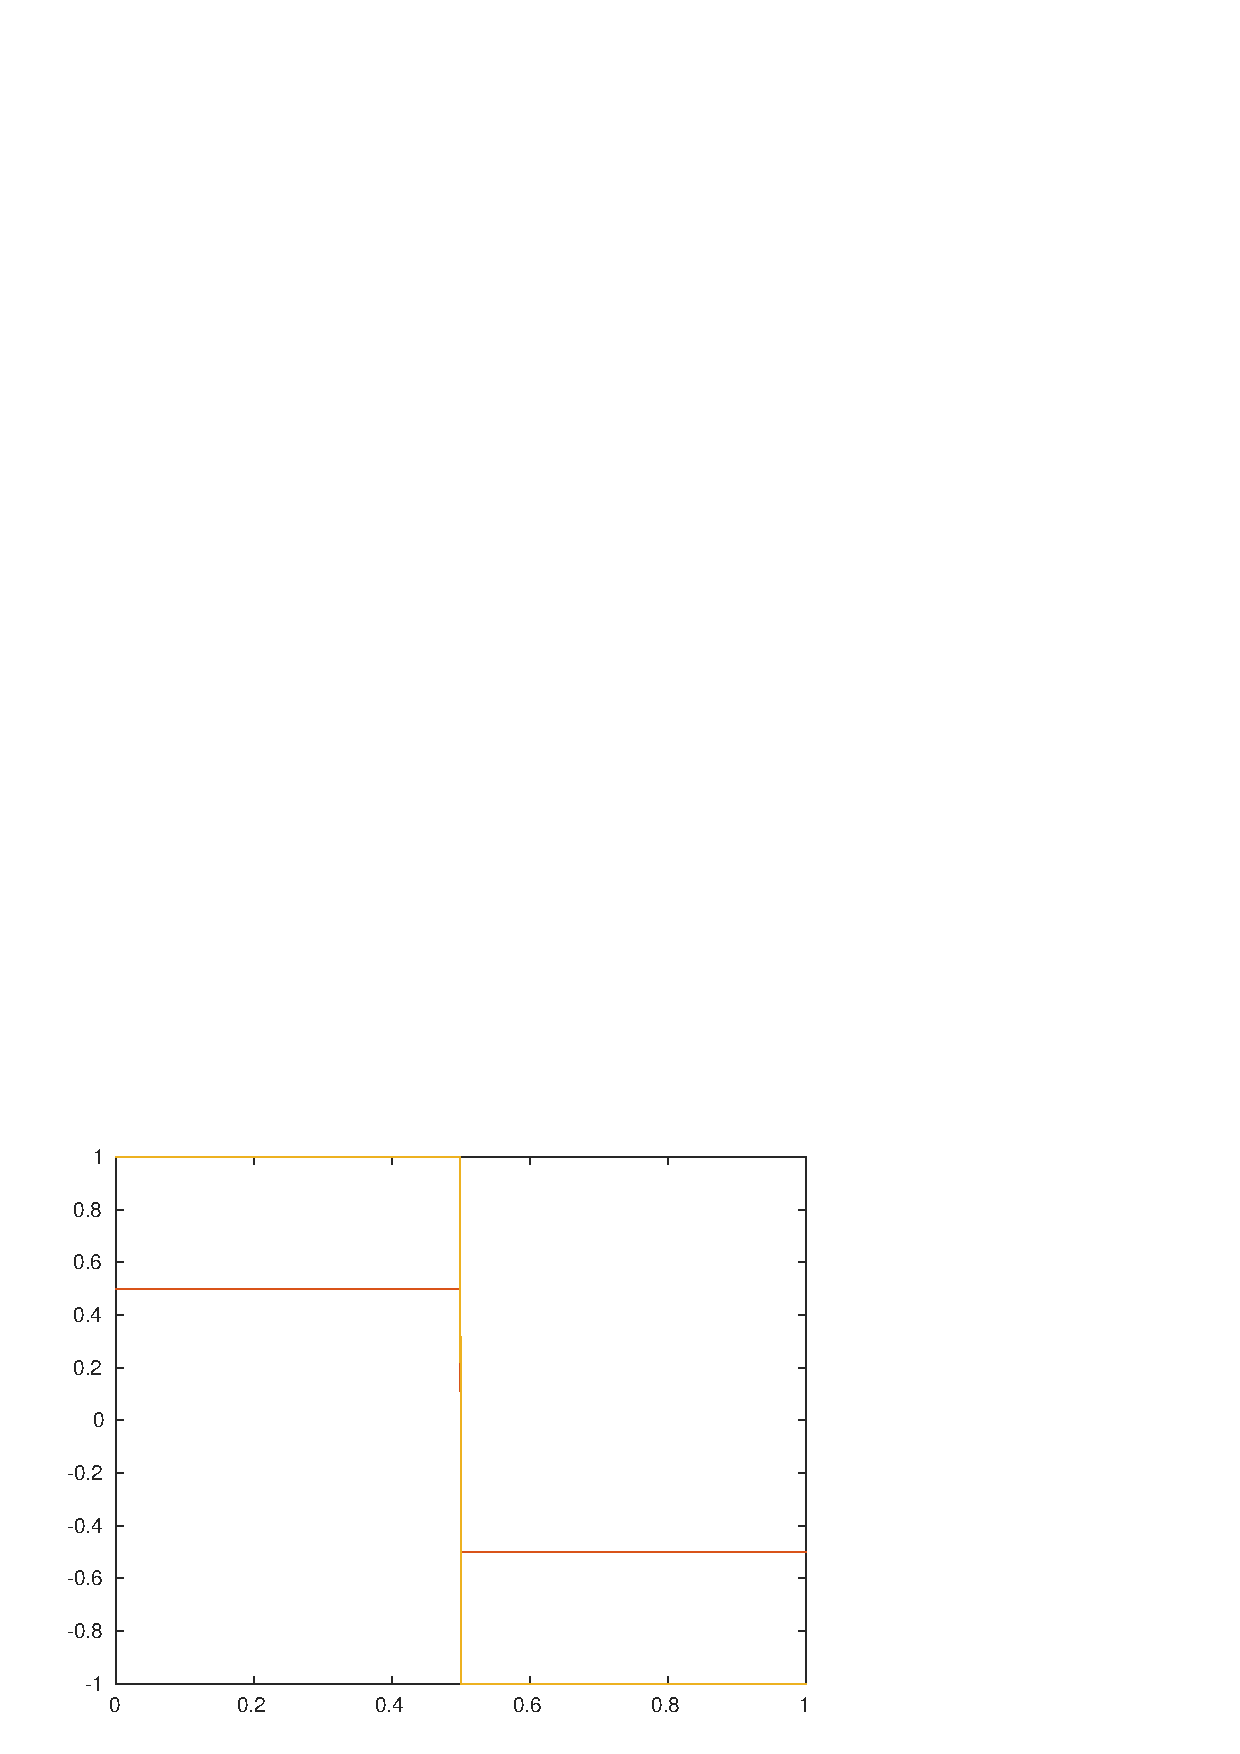
\includegraphics[width=10cm]{1.pdf}
\caption{開球体$\bs(p,1)$を表す領域\newline
	{\footnotesize A,B,O,P四点共線,点A,Bを含まない,文字fを無視せよ.$\de(A,P)=\de(P,B)=1$である}}
\end{figure}
\begin{figure}[H]
\centering
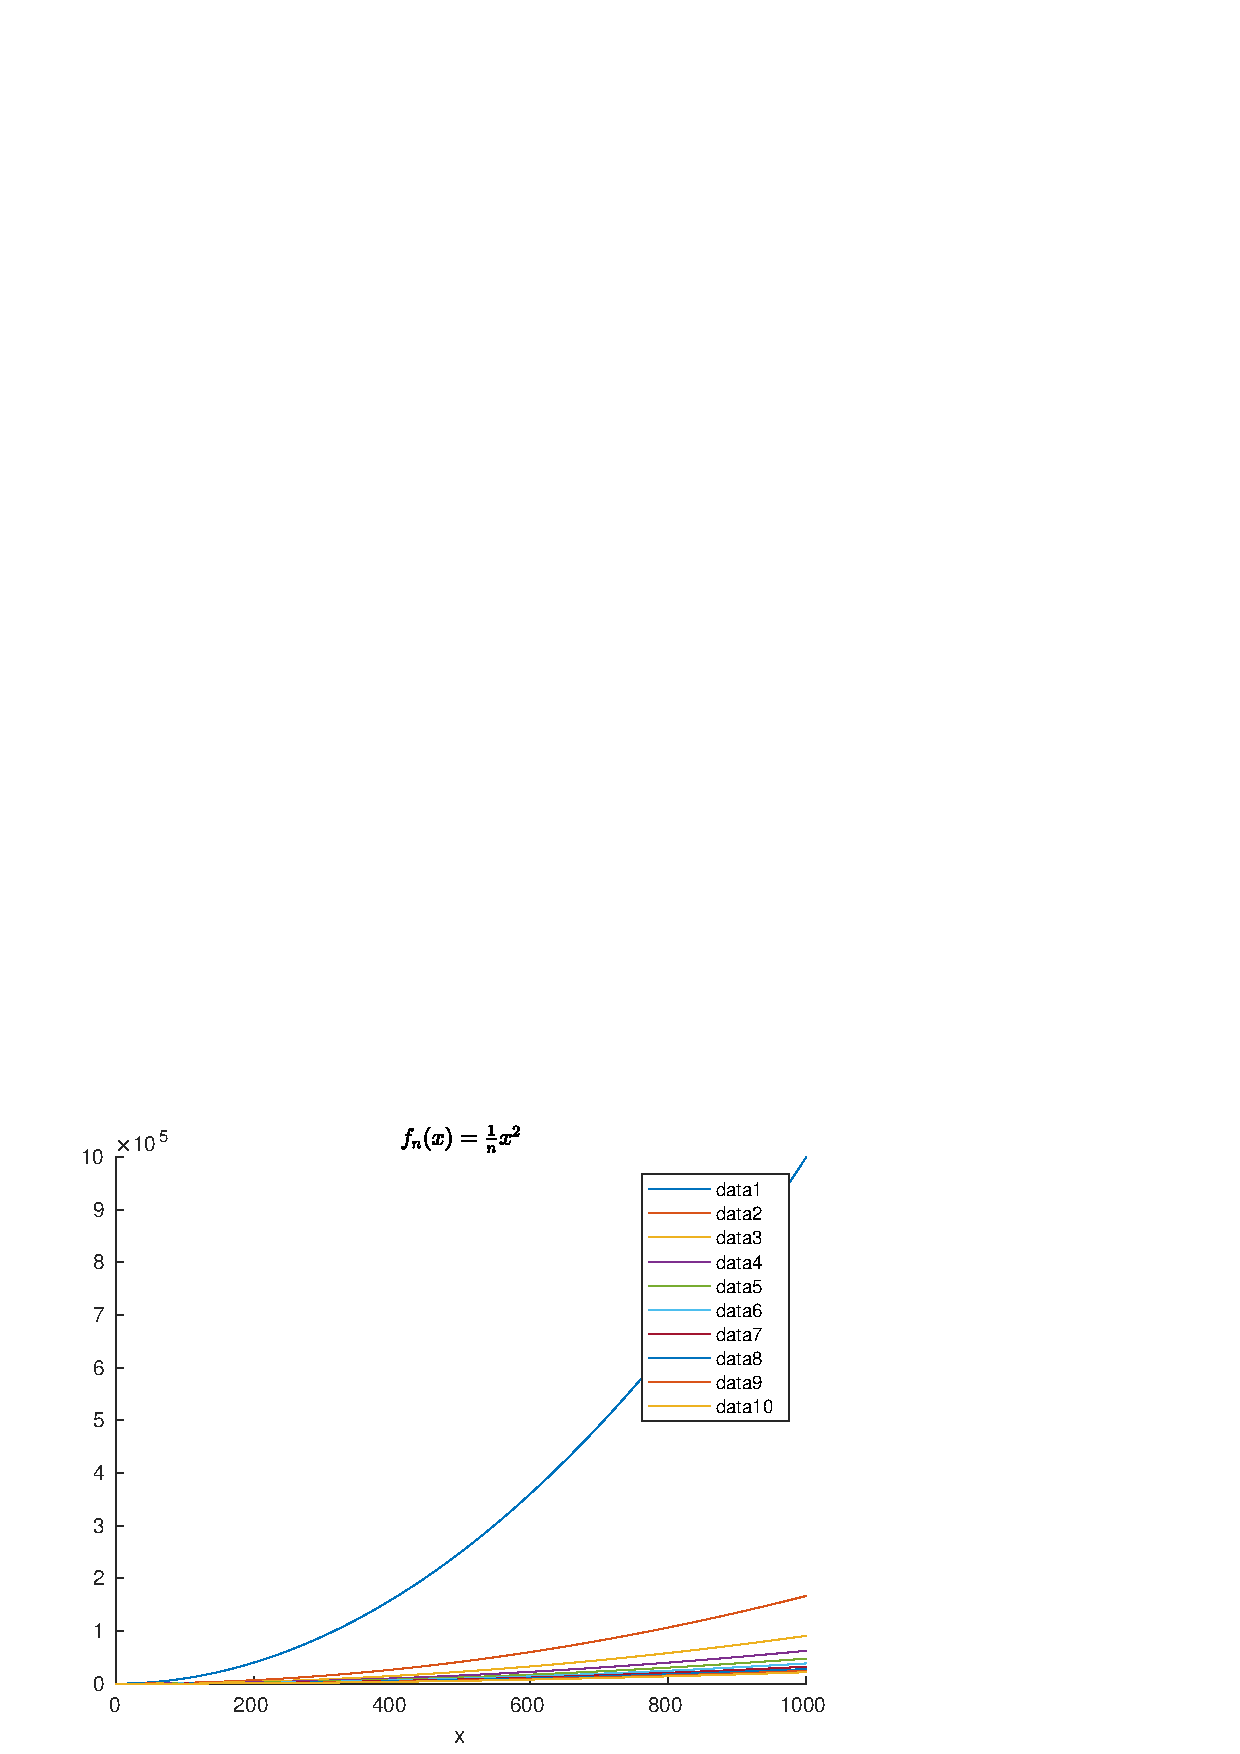
\includegraphics[width=10cm]{2.pdf}
\caption{開球体$\bs(p,2)$を表す領域\newline
	{\footnotesize A,B,O,P四点共線,点A,Bを含まない,文字fを無視せよ.$\de(A,P)=\de(P,B)=2$である}}
\end{figure}
\begin{figure}[H]
\centering
\includegraphics[width=10cm]{3.pdf}
\caption{開球体$\bs(p,2.1)$を表す領域\\
	{\footnotesize A,B,O,P,C四点共線,点B,Cを含まない,文字gを無視せよ$\de(P,B)=\de(P,C)=2.1,\de(B,O)=0.1$である}}
\end{figure}
\begin{figure}[H]
\centering
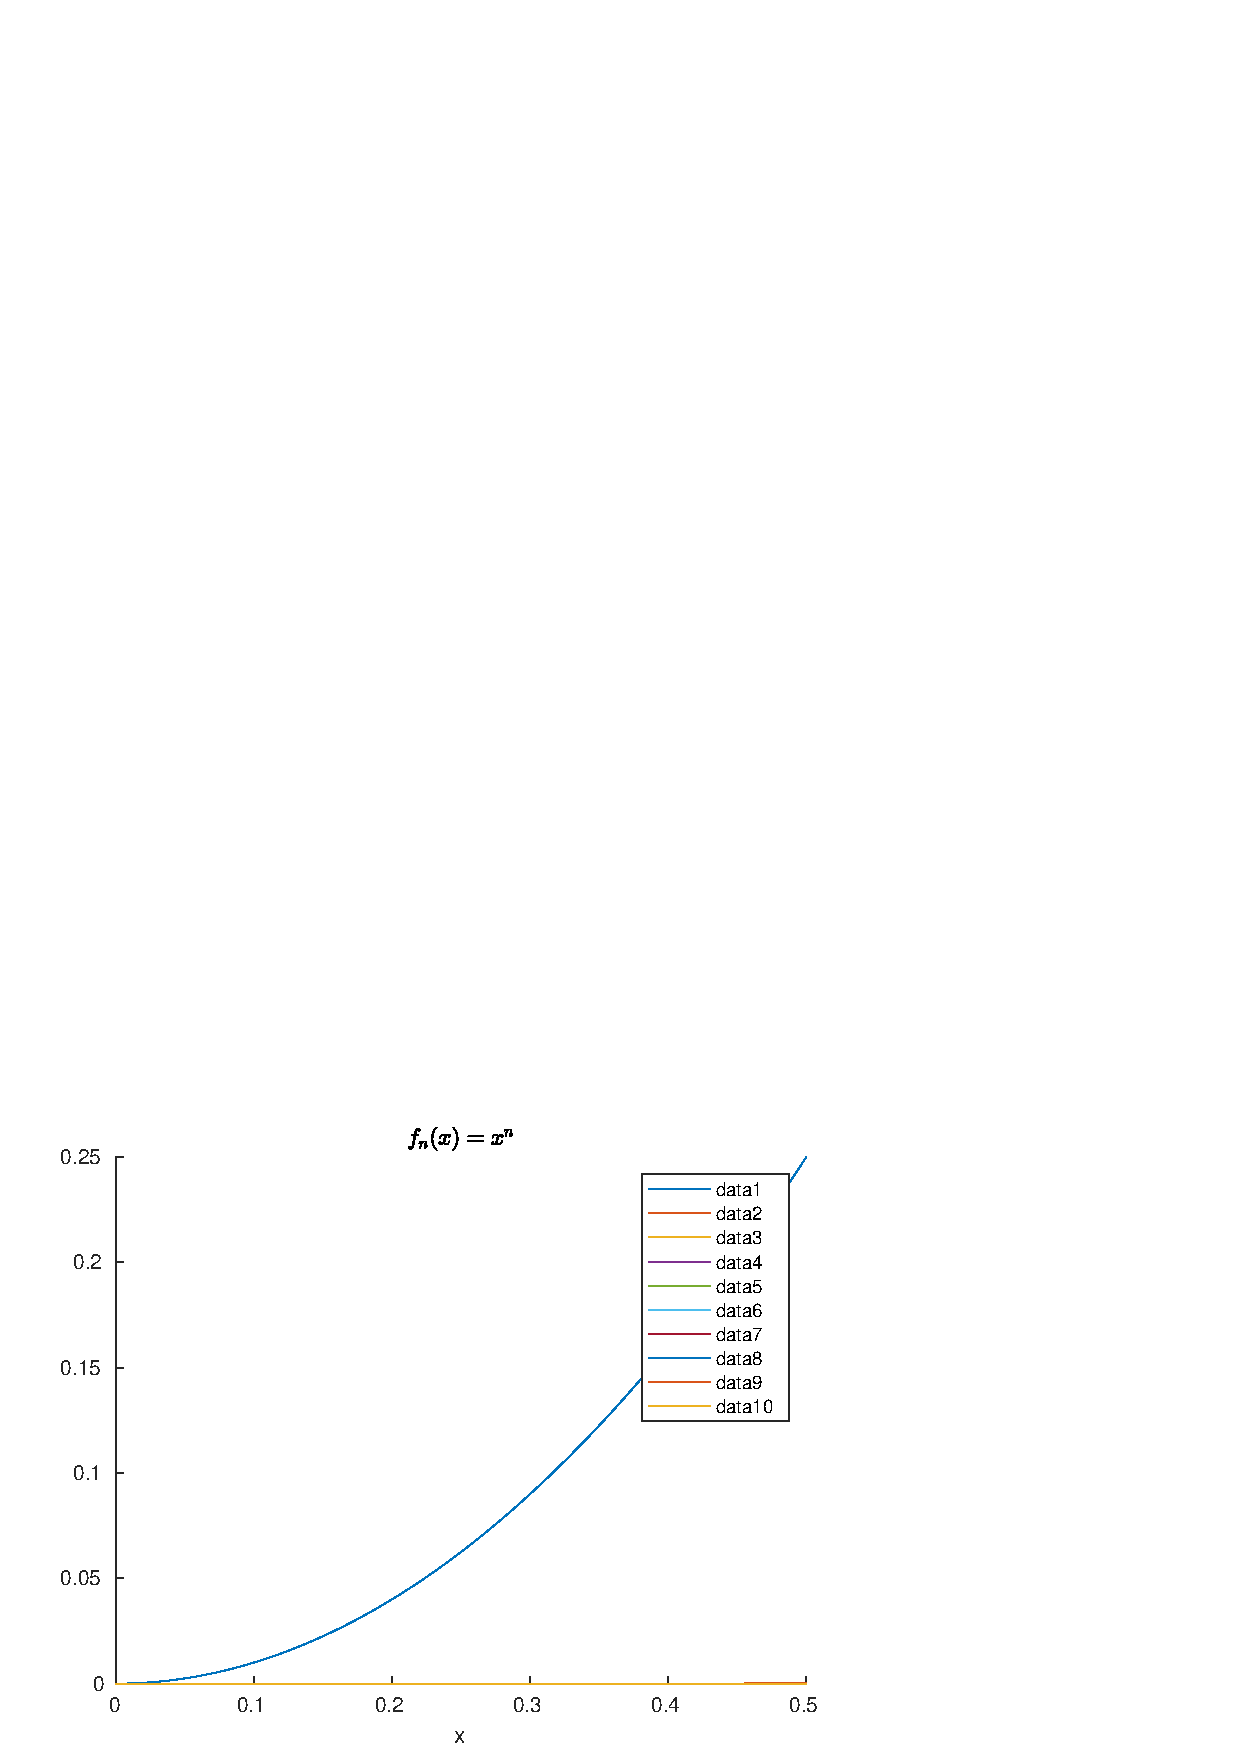
\includegraphics[width=10cm]{4.pdf}
\caption{開球体$\bs(p,3)$を表す領域\\
	{\footnotesize A,B,O,P,C四点共線,点B,Cを含まない,文字gを無視せよ$\de(B,P)=\de(P,C)=3,\de(B,O)=1$である}}
\end{figure}
\newpage

\subsubsection{(2)集合C,D,Eについて,判定を行え}
\textcolor{red}{集合$C$は開集合でない}
\begin{proof}
集合$C$の要素$o$を取る.$r \in \Rp$を任意に取る.この時,点$q=(0,r/2)$とする.開球体$\bs(o,r)$に対し,$\ds(o,q)=r/2 <r$より,$q \in \bs(o,r)$が得られる.
しかし,$0^2-3(r/2)^2<0$より,$q \notin C$,従って,$\bs(o,r) \not\subseteq C$が成立する.\\
以上より,集合$C$は距離空間$(\R^2,\ds)$の開集合ではないことが示された.
\end{proof}
\textcolor{red}{集合$D$は閉集合ではない}
\begin{proof}
集合$D$は閉集合ではないことを示すには,集合$\R^2 \setminus D =\{(x,y) \in \R^2 \mid x^2+y^2 \ge 1\}$が開集合でないことを示せば良い.\\
集合$\R^2 \setminus D$は開集合でないことを以下示す:\\
点$p=(1,0)$とする.この時,$p \in \R^2 \setminus D$であることは明らかである.この点$p$に対し,$r \in \Rp$を任意に取る.\\
この場合,実数$q=\max\{1-r/2,1/2\}$と定め,点$b=(q,0)$とする.\\
$\ds(p,b)=\de(p,b) \le r/2 <r$より,$b \in \bs(p,r)$が成立する.しかし,$q^2+0^2 \le 1/4 <1$より,$b \notin \R^2 \setminus D$が得られる.\\
従って,開球体$\bs(p,r) \not\subseteq \R^2 \setminus D$となり,集合$\R^2 \setminus D$は開集合でないことがわかる.\\
以上より集合$D$が閉集合でないことを示せた.
\end{proof}
\textcolor{red}{集合$E$は開集合である}
\begin{proof}
$$
\forall x \in E; \exists r \in \Rp ; \bs(x,r) \subseteq E
$$
上記の論理式が成立することを以下示す:\\
$x \in E$を任意に取る,$x \in D$と$x \notin D$について場合分けして議論する.\\
$x \in D$の時,実数$r = \frac{1}{4}(1-\ds(x,o))$とする.この時,点$q=(a,b) \in \bs(x,r)$を任意に取る.\\
$$
\begin{aligned}
a^2+b^2 &= \de(o,q) \le \ds(o,q)  \\
        &\le  \ds(o,x) +\ds(x,q) \le \ds(o,x) +r \\
	&\le \frac{1}{4}(1+3\ds(o,x))
\end{aligned}
$$
この時,$x \in D $より,$\ds(o,x)=\de(o,x)<1$が得られ,$a^2 +b^2<1$となり,点$q \in D$であることが示された.\\
つまり,$\bs(x,r) \subseteq D \subseteq E$が成立する.\\
$x \notin D$の時,点$x=(m,n)$とする.この場合,$\ds(o,x) \ge \de(o,x) \ge 1$が成り立つ.また$x \in C$より,$(m=\sqrt{3}n) \lor (m=-\sqrt{3}n)$が常に成り立つ.
実数$r = \frac{1}{2}$とする.この時,点$q=(a,b) \in \bs(x,r)$を任意に取る.以下$q \notin C$と仮定して,矛盾を導く:\\
仮定より,$(a \neq \sqrt{3}b ) \land (a \neq - \sqrt{3}b)$が成り立つ.この時,$x,q,o$が同一直線上にないことがわかる.\\
この場合,$\ds(x,q)=\de(x,o)+ \de(o,q)$が得られ,しかし,$\ds(x,q)<\frac{1}{2}<1\le \de(x,o)+\de(o,q)$,これで,矛盾が生じ,$q \in C$が成り立つことを示せた.\\
つまり,$\bs(x,r) \subseteq C \subseteq E$が成立する.\\
以上の場合分けの議論より,$\forall x \in E; \exists r \in \Rp ; \bs(x,r) \subseteq E$が得られる.\\
従って,集合$E$は距離空間$(\R^2, \ds)$の開集合である.
\end{proof}
\newpage
\subsubsection{(3)写像$\Phi : (\R^2,\ds) \to \R$が連続であるかどうかを判別せよ}
\textcolor{red}{連続である}\\
本問において,$x\neq o$を満たす,$x \in \R^2$を一意的に存在する実数$r_x \in \Rp ,\theta_x \in [0,2\pi)$で$x=(r_x\cos\theta_x,r_x\sin\theta_x)$と書く操作を極表示とする.
\begin{proof}
	$x \in (\R^2, \ds)$を任意に取る.この時,$x = o$と$x \neq o$について場合分けして議論を行う:\\
	$x = o$の時,$\varepsilon \in \Rp$を任意に取る.この時,$\delta = \frac{\varepsilon}{4 \pi}$とする.開球体$\bs(x,\delta) = \{ (a,b) \in \R^2 \mid \sqrt{a^2+b^2} < \delta  \}$である.\\
	次に,$\ds(x,x')<\delta$を満たす$x' \in R^2$を任意に取る.開球体の定義より,$x' \in \bs(x,\delta)$が成り立つ.実数$r_{x'} \in \Rp\cup\{0\} ,\theta_{x'} \in [0,2\pi)$を用いて,$x'$を$(r_{x'}\cos\theta_{x'} , r_{x'}\sin\theta_{x'})$とする\footnote{($x' \neq o$の時,$r_{x'},\theta_{x'}$が両方共に一意的に決まる.$x'=o$の時,$\theta_{x'}$が一意的に決まらないが,$r_{x'}=0$が必ず成り立つので,次の議論は破綻しない)} .\\
	$x' \in \bs(x,\delta)$より,$r_{x'} < \delta$が得られる.この時,$|\Phi(x) -\Phi(x')| = |\Phi(x')|\le 2\pi \cdot r_{x'} \le 2\pi \delta < \varepsilon$が成立する.\\
	続いて,$x \neq o$の時,実数$r_x \in \Rp,\theta_x \in [0,2\pi)$が一意的に存在し,$x=(r_x \cos\theta_x,r_x \sin\theta_x)$と書ける.この実数$r_x,\theta_x$を取る.次に$\varepsilon \in \Rp$を任意に取る.この時,$\delta =\min\left\{ \frac{1}{4}\cdot \ds(o,x), \frac{\varepsilon}{4\pi} \right\}$とする.\\
	今,開球体$\bs(x,\delta)=\left\{ x' \in \R^2 \mid x'を極表示した時, \theta_{x'} =\theta_x, |r_{x'}-r_x|<\delta \right\}$となる\footnote{($\ds(o,x)>\delta$より,$o\notin \bs(x,\delta)$,よって,集合内の$x'$に関する表記がwell-definedである)}.従って,$\ds(x,x')<\delta$を満たす$x' \in \R^2$を任意に取った時,$x' \in \bs(x,\delta)$が成立するので,$|\Phi(x) - \Phi(x')|\le \theta_x |r_x- r_{x'}|<2\pi \cdot \delta <\varepsilon$が得られる.\\
	以上より,
	$$
	\forall x \in \R^2; \forall \varepsilon \in \Rp ; \exists \delta \in \Rp; \forall x' \in \R^2;\left( \ds(x,x')<\delta \implies \de(\Phi(x),\Phi(x'))<\varepsilon \right)
	$$
	が成立することを示せた.つまり,写像$\Phi : (\R^2,\ds) \to \R$が連続である.
\end{proof}
\newpage
\section{リーマン広義可積分な連続函数のなす空間について}
本問では,実数$x$に対し,$N(x)$を$x$以上の最小の自然数とする.
\subsection{$(V,d_1)$が距離空間であることを示せ}
\begin{proof}
$f,g,h \in V$を任意に取る,集合$V$がベクトル空間であることより,$f-g\in V,f-h \in V,h-g \in V$が成立する.\\
この時,(a1)より,$d_1(f,g) = \| f-g \|_1 \ge 0$\\
次に$d_1(f,g) = \| f-g \|_1 =0$が成立するならば,(a2)より,$f-g=0$が成立する.つまり,$\forall x \in \R; f(x) =g(x)$で,$f=g$が得られる.\\
また,$d_1(f,g) = \|f-g\|_1= \int_{\R}|f(t)-g(t)|dt= \int_{\R}|g(t)-f(t)|dt=\|g-t\|_1=d_1(g,f)$が成立する.\\
最後に,(c)より$d_1(f,g) = \| f-g\|_1= \|(f-h)+(h-g)\|_1 \le \|f-h\|_1 +\|h-g\|_1 = d_1(f,h) + d_1(h,g)$も成立する.\\
以上より,写像$d_1$は非負性,分離性,可換性,三角不等式を満たしているため,集合$(V,d_1)$は距離空間であることを示せた.
\end{proof}
\newpage
\subsection{点列$(h_n)_{n \in \mathbb{N}}$が$(V,d_1)$上のCauchy列であることを示せ}
\begin{proof}
	$\varepsilon \in \Rp$を任意に取る.この時,$N=\max\{100,N(\frac{4}{\varepsilon}) \}$とする,$m,n \ge N$を満たす自然数$m,n$を任意に取る.\\
	$$
	\begin{aligned}
		d_1(h_m,h_n) &=\|h_m - h_n\|_1 = \int_{\R} |h_m(t) - h_n(t) |dt = \int_{-1}^{1} \left| \frac{t^{2n} - t^{2m}}{1+t^{2022}} \right| dt\\
			     &\le 2 \int_0^1 t^{2N}  \left( \left| \frac{1^{2(n-N)}}{1+0^{2022}} \right| + \left| \frac{1^{2(m-N)}}{1+0^{2022}} \right| \right)dt\\
			     &\le 4 \int_0^1 t^{2N} dt \le \frac{4}{2N+1} <\varepsilon
	\end{aligned}
	$$
	以上より,点列$(h_n)_{n \in \mathbb{N}}$が$(V,d_1)$上のCauchy列であることを示せた.
\end{proof}
\newpage
\subsection{$(V,d_1)$は完備距離空間であるかどうかを判定せよ}
\textcolor{red}{完備距離空間ではない}
\begin{proof}
$(V,d_1)$上の任意のCauchy列が$(V,d_1)$の一点に収束すると仮定して,このもとで矛盾を導く.\\
前問におけるCauchy列$(h_n)_{n \in \mathbb{N}}$を取る.仮定より,点列$(h_n)_{n \in \mathbb{N}}$が点$h \in V$に収束する,この点$h$を取る.\\
	各自然数$n$に対し,$h_n$は$\R$上の連続かつリーマン可積分の函数であることより,$h_n$は$A=(-\infty,-1)\cup (1,\infty),B=[-1,1]$においても連続かつリーマン可積分である.\\
函数$g: A \to \R$,函数$z: B \to \R$を次のように定める:\\
\begin{align}
	g(x) &=0\\
	z(x) &=\frac{1}{1+x^{2022}}
\end{align}
この時,点$h$に対し,以下の条件が成り立つ:
	\footnote{	この時,函数列$(h_n)_{n\in \mathbb{N}}$は集合$A$で函数$g$に一様収束し,集合$B\setminus\{\pm 1\}$で函数$z$に各点収束する.前半は引き算により自明である,後半は任意に与えたれた$x,\varepsilon$に対し,$x^{2N}<\varepsilon $を満たす自然数$N$が存在することより簡単に示せる.} \\
$$
h(x) = 
\begin{cases}
	0,x\in A\\
	\frac{1}{1+x^{2022}} ,x \in B
\end{cases}
$$
仮に上記の条件が成り立たないとすると,ある正の実数$\varepsilon_0$が存在し,
$$
\int_A | h(x) -g(x)|dx + \int_B |h(x) -z(x)|dx = \varepsilon_0 
$$
を満たす.しかし,$\varepsilon_0$に対し,ある自然数$N'$が存在し,$n\ge N'$を満たす$n\in\mathbb{N}$について,$d_1(h,h_n)<\varepsilon/8$が成り立つ.このような$N'$を一つ取り,$N = \max \{ N',N(\frac{32}{\varepsilon_0}) \}$
とする.\\
$$
\begin{aligned}
	\varepsilon_0&= \int_A | h(x) -g(x)|dx + \int_B |h(x) -z(x)|dx\\
	&\le \int_A |h(x) - h_N(x)|dx + \int_A | h_N(x) -g(x)|dx \\
	& \quad+\int_B|h(x)-h_N(x)|dx + \int_B|h_N(x)-z(x)|dx\\
						       &\le 3 \times \frac{\varepsilon_0}{8} + 2\int_0^1 t^{2N}dt \le 4\times \frac{\varepsilon_0}{8} =\frac{\varepsilon_0}{2}
\end{aligned}
$$
これで矛盾が生じる.よって,点$h$について,次の条件を満たさなければいけない:
$$
h(x) =
\begin{cases}
        0,x\in A\\
	\frac{1}{1+x^{2022}} ,x \in B
\end{cases}
$$
この場合,$x =1$において,$h$は連続でないことを示せる:\\
$\varepsilon = |h(1)|/2$とする.$\delta \in \Rp$を任意に取る.この場合,$x=1+\delta/2$とする.$|x-1|<\delta$が成り立つが,$|h(x)-h(1)| = |h(1)|>\varepsilon$となるので,連続でないことが得られる.\\
以上より$h$が$\R$上の連続函数ではないことが示され,$h \notin V$がわかる.従って,矛盾が生じ,$(V,d_1)$が完備距離空間ではないことを示せた.
\end{proof}
\newpage
\section{\# 雑談}
あけましておめでとうございます.残りの付き合いもそんなに長くならないと思いますがとりあえず今年もよろしくお願いします.いよいよ序論の最終のレポートになりました.最後のレポートのレポートは今まで一番難しいと予想したけど,実際に解いたらそうではないような気がします.今回はかなりの力を入れて添字ミスを確認したので,第四回みたいな悲惨な状況にならないだろう.正直,今回のレポートに関して,開球体を定式化して表現する際に,求める過程も入れるかどうかに迷っていました.しかし,余計に書くと文が長くなり,読みやすいとは言えなくなります.ですので,開球体の式,距離の計算,定積分の評価などに関しては,最初の部分だけアイデアを明示して丁寧に示していく.それ以降の部分は似たような計算や評価方法を採用していただければ,同じような結論に至るはず.\textcolor{red}{\sout{以上を以て,一年次の数学序論のレポートを終了とさせてい\linebreak ただきます.期末試験は対面で受ける予定ですから,この記述もwell-defined\linebreak である.}}長い時間採点者として付き合ってくださり,まことにありがとうございます.では雑談を終了したいと思います,また期末レポートの採点作業でお会いしましょう.今まで長い時間取らせていただき,お疲れ様でした.







\end{document}

